

\section{Sèries temporals}
\label{sec:art:seriestemporals}



Una sèrie temporal és un conjunt de valors cadascun dels quals té
associat un instant de temps diferent.  Tradicionalment s'anomenen
sèries temporals tot i que també s'accepta la denominació de
seqüències temporals, per exemple a \cite{last:hetland}.

Les sèries temporals s'emmarquen dins l'àmbit més genèric del que es
coneix com a \emph{dades temporals}. Les dades temporals són
co\l.leccions de dades arbitràries que estan associades a la dimensió
temps.  Dins del concepte de dades temporals s'hi encabeixen
co\l.leccions de dades de diversa natura. En funció de com un valor
queda vinculat amb el temps, es poden diferenciar dues
categories \parencite{assfalg08:thesis}.
\begin{enumerate}
\item La primera la formen les sèries temporals tal i com s'han
  definit prèviament, en la qual la dada està associada a un instant
  de temps.
\item La segona, que s'anomena dades bitemporals (\emph{bitemporal
    data}), la formen co\l.leccions de dades en què cada element té
  dos atributs temporals: el rang de validesa, que indica l'interval
  de temps en que la dada és vàlida, i el temps de transacció, que
  indica quan es va desar la dada a la base de dades.
  %\citeauthor{assfalg08:thesis} a \cite{assfalg08:thesis} assegura que aquesta categoria de dades temporals es poden expressar en termes de la primera.\todo{Teresa5}
\end{enumerate}
Aquestes dues categories de dades temporals, tot i tenir aspectes en
comú, no poden ser tractades amb els mateixos
sistemes, \parencite{schmidt95}.


Les sèries temporals s'utilitzen en camps molt diversos i amb
objectius molt diferents. L'ús generalitzat és per a l'anàlisi i la
comprensió del comportament temporal de variables. L'evolució d'una
sèrie temporal es pot representar amb un model. Aquests models, en
l'àmbit de l'enginyeria, permeten realitzar tasques relacionades amb
validació de dades, diagnòstic i prognosis.  Per exemple, trobem
aplicacions de sèries temporals en el camp de l'avaluació de la
degradació de components \parencite{yu11}, anàlisi de l'estat dels
sensors d'un vaixell \parencite{palmer07}, validació i reconstrucció
de dades en xarxes de distribució d'aigua \parencite{quevedo10},
classificació de valors econòmics \parencite{dreyer95}, optimització
de la planificació semafòrica \parencite{last11}, estimació del temps
de viatge en autopistes \parencite{soriguera10} o transmissió
d'informació en xarxes de
sensors \parencite{jainagrawal05,yaogehrke02}.
% \todo{també sèries temporals van de bracet amb SIG, exemple en dades hidrològiques [bollaert06:thesis]}


Aquest apartat té com a objectiu mostrar l'estat de l'art dels
principals processos vinculats en el treball amb sèries temporals. A
tal efecte s'organitza en tres subapartats.
 


El primer subapartat tracta de l'anàlisi de sèries temporals, que és
la formalització de les tècniques que s'utilitzen per extreure
informació. A vegades aquesta extracció també es coneix com
descobriment de coneixement i es pot emmarcar dins de l'inte\l.ligència
artificial.


El segon subapartat se centra en l'adquisició de dades. El primer
requeriment d'una sèrie temporal és l'adquisició de dades. Els
sistemes de monitoratge s'encarreguen de recollir dades dels sensors,
periòdicament o en base a esdeveniments.  Els problemes que es donen
durant l'adquisició generen defectes específics en les sèries
temporals que cal analitzar i tractar convenientment.


El tercer subapartat es dedica als sistemes d'emmagatzematge de sèries
temporals. L'emmagatzematge de les dades i la implementació de les
tècniques d'anàlisi ocorre en els \glspl{SGBD}. Aquests s'encarreguen
de l'organització correcte de la informació i de respondre a les
operacions de consulta. Les sèries temporals necessiten un tractament
específic per part d'aquests sistemes.



\subsection{Anàlisi de sèries temporals}


% explicar el data mining com a background per a les oepracions que es poden fer amb les sèries temporals: pattern search, similiraties, etc.


L'anàlisi de sèries temporals consisteix en l'aplicació de
metodologies i d'algoritmes que permeten tasques com per exemple
l'extracció de característiques o obtenció de models.  Aquestes
tècniques es recullen en el que es coneix amb el nom de mineria de
sèries temporals (\emph{time series data mining}). La mineria de
dades, en la qual s'inscriu la de sèries temporals, és l'estudi
d'algoritmes específics per a extreure patrons de comportament de les
dades i s'inclou com un pas del procés general de descobriment de
coneixement a les bases de dades (\emph{knowledge discovery in
  databases}) \parencite{fayyad96,last01}

% [M. E. Mueller, Relational Knowledge Discovery, Cambridge 2012. sec1.1p7]
%knowledge discovery: process of extracting new knowledge from a set of data about that set of data, This means that the acquisition of new lnowledge requires us to build a new model of the data.
% Data mining: refers mostly to the extraction of parts of information with respect to a given model. 
%Exemple: correlació, si dues coses tenen correlació no vol dir que necessàriament hi hagi una dependència causal entre les dades.

Actualment, les sèries temporals es consideren com un dels deu problemes
prioritaris en la mineria de dades \parencite{yangwu06}. Tal com
esmenta \textcite{fu11} en un article recent, la recerca en mineria de
sèries temporals s'ha incrementat en la darrera dècada. L'objectiu
principal és reduir la mida de les sèries temporals per tal de
disminuir el temps de processat de les dades.  \citeauthor{fu11}
resumeix l'estat actual de la mineria de sèries temporals de forma
exhaustiva i conclou que encara queden molts problemes per investigar
i resoldre. La recerca en tasques de mineria ha estat intensa però es
necessita millorar la representació de sèries temporals, ja que es
considera el pas que redueix la mida de les dades.

Segons \textcite{keogh02}, les quatre tasques que centren l'atenció de
la recerca actual de sèries temporals són l'indexat (\emph{indexing}),
que treballa amb una estructura comprimida de les dades; l'agrupament
(\emph{clustering}), que agrupa les dades segons la similitud entre
elles per tal de descobrir patrons; la classificació
(\emph{classification}), que etiqueta les dades segons les
característiques que presentin; i la segmentació
(\emph{segmentation}), que parteix una sèrie temporal en
subseqüències.  A més, \citeauthor{keogh02} comparen alguns algoritmes
experimentals duts a terme en aquests camps per diversos
autors. Recomanen a la comunitat de mineria de sèries temporals que
segueixi el seu estudi com a punt de referència per avaluar el
rendiment d'algoritmes similars.



Un pas comú previ a les quatre tasques anteriors és el de
representació de la sèrie temporal. Les sèries temporals són
discretes, són valors en punts de temps discrets, i la representació
és el model de funció que aproxima la sèrie temporal a la seva
naturalesa contínua original. La mineria de sèries temporals aprofita
la representació per reduir la mida de les sèries temporals. 



\textcite{last:keogh}, cita vàries representacions per les sèries
temporals com per exemple \emph{Fourier Transforms}, \emph{Wavelets},
\emph{Symbolic Mappings} o \gls{PLR}, però assenyala aquesta última
com la representació més utilitzada.  La
\gls{PLR} \parencite{keogh97,keogh98} és una representació definida a
trossos lineals que s'aproxima a la sèrie temporal. Els trossos
podrien ser polinomis de qualsevol grau, però la manera més comuna de
representar sèries temporals és amb funcions lineals ja que és més
propera a la visió de l'ésser humà que segmenta les corbes en línies
rectes.  A banda de la \gls{PLR}, \textcite{keogh00,keogh01} exploren
altres representacions de sèries temporals per tal de reduir la mida
d'una sèrie temporal i poder-la indexar més fàcilment. Proposen dues
tècniques eficients en el càlcul: la \emph{Piecewise Aggregate
  Aproximation} i la \emph{Adaptive Piecewise Constant Approximation},
ambdues basades en la representació a trossos constants de la sèrie
temporal.  D'aquestes dues tècniques, \citeauthor{keogh00,keogh01}
conclouen que mantenen una bona aproximació a la sèrie temporal i que
a més tenen molt menys cost de càlcul que altres de més complicades,
com ara la \emph{Discrete Fourier Transform}, la \emph{Singular Value
  Decomposition} o la \emph{Discrete Wavelet Transform}.

Altres representacions també aproximen una sèrie temporal a trossos
però generalitzen la funció d'aproximació. Per exemple
\textcite{last01} proposa aproximar una sèrie temporal partint-la en
subintervals i calculant per a cada un la funció que més s'hi
aproxima.  Un altre àmbit on s'aplica l'anàlisi de sèries temporals és
en teoria del senyal.  Aleshores també podem utilitzar les
representacions habituals en teoria del senyal, per exemple es pot
representar una sèrie temporal amb una funció graó (\emph{step} o
\emph{staircase function}); és a dir, amb una funció definida a
trossos constant (\emph{piecewise constant representation}).


% Per aproximar el segment $S(t_a,t_b]$ d'una sèrie $S$, Keogh defineix dues tècniques: interpolació lineal, la recta que connecta $t_a$ i $t_b$, i regressió lineal, la millor recta que aproxima per mínims quadrats el segment entre $t_a$ i $t_b$ \parencite{keogh02}.



% \paragraph{Representació de sèries temporals}

% Però també es pot representar una sèrie temporal amb una funció graó (\emph{step} o \emph{staircase function}); és a dir, amb una funció definida a trossos constant (\emph{piecewise constant representation}).
% La representació a trossos constant és utilitzada en electrònica als convertidors digital-analògic (DAC, \emph{digital-to-analog converter}). En aquest cas, un senyal discret es considera una sèrie temporal i per reconstruir el senyal continu típicament s'aplica el model de \emph{zero-order hold}, equivalent a la representació a trossos constant,  o el de \emph{first-order hold},  equivalent a la representació a trossos lineal.
% El model de \emph{zero-order hold} consisteix en mantenir constant cada valor fins al proper. S'obté una representació a trossos constant que en electrònica s'anomena seqüència de pulsos rectangulars (\emph{rectangular pulses}).

%http://en.wikipedia.org/wiki/Piecewise

%http://ca.wikipedia.org/wiki/Funció_definida_a_trossos

%http://en.wikipedia.org/wiki/Rectangular_function

%http://en.wikipedia.org/wiki/Step_function

% Piecewise Aggregate Approximation (PAA) \cite{keogh00}: aproxima una sèrie temporal partint-la en segments de la mateixa mida i emmagatzemant la mitjana dels punts que cauen dins del segment. Redueix de dimensió $n$ a dimensió $N$

% Adaptive Piecewise Constant Approximation (APCA) \cite{keogh01}: com el PAA però amb segments de mida variable.






\subsection{Adquisició i monitoratge de sèries temporals}

Els sistemes de monitoratge són una part important d'interacció entre
un procés i els usuaris, entenent com a procés qualsevol sistema
físic, químic, ambiental, etc.\ del qual es pugui recollir informació
continuada, ja sigui de forma periòdica o en funció
d'esdeveniments. Principalment, aquests sistemes s'encarreguen de
recollir dades, conèixer l'estat actual del procés i informar a
l'usuari. Els sistemes de monitoratge constitueixen la part principal
dels \glspl{SCADA}. Un \gls{SCADA} és un sistema encarregat de recollir i
centralitzar les dades de manera periòdica en el temps.



\begin{figure}[tp]
  \begin{center}
    \scriptsize 
    \usetikzlibrary{arrows,positioning}
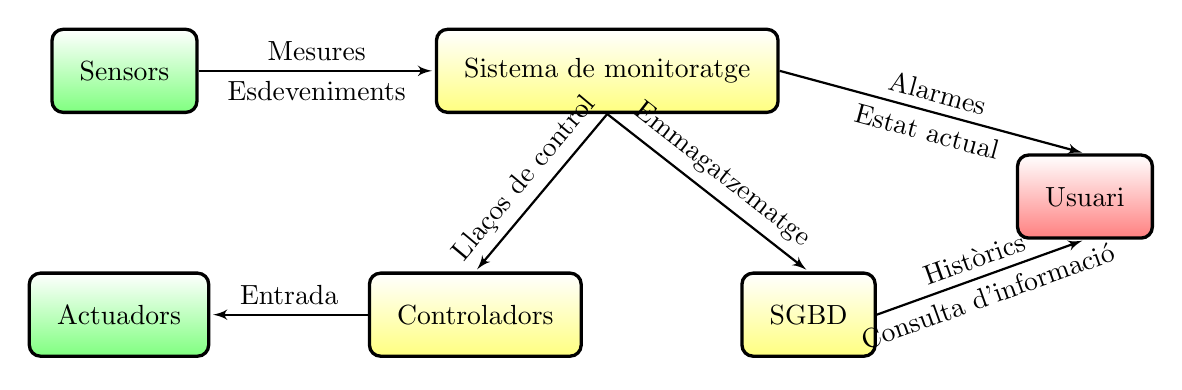
\begin{tikzpicture}[node distance=0.5cm]  
  \tikzset{
    mynode/.style={rectangle,rounded corners,draw=black, 
      very thick, inner sep=1em, minimum size=3em, text centered,
      groc},
    myarrow/.style={->, >=latex', shorten >=1pt, thick},
    mylabel/.style={text width=7em, text centered},
    groc/.style={top color=white, bottom color=yellow!50},
    verd/.style={top color=white, bottom color=green!50},
    roig/.style={top color=white, bottom color=red!50},
  }  

  \node[mynode]                                       (monitor)   {Sistema de monitoratge};  
  \node[mynode, below right=2cm and -0.5cm of monitor]  (bd)        {SGBD}; 
  \node[mynode, below=2cm of monitor, left=2cm and 2cm of bd]     (control)   {Controladors}; 
  \node[mynode, roig, below right=0.5cm and 3cm of monitor] (usuari)    {Usuari};  
  \node[mynode, verd, left=2cm of control]            (actuador)  {Actuadors};
  \node[mynode, verd, left=3cm of monitor]            (sensor)    {Sensors};  


  \draw[myarrow] (monitor.east) --   (usuari.north)	
     node [above,sloped,midway] {Alarmes}
     node [below,sloped,midway] {Estat actual};
  \draw[myarrow] (bd.east) --   (usuari.south)
     node [above,sloped,midway] {Històrics}
     node [below,sloped,midway] {Consulta d'informació};
  \draw[myarrow] (sensor.east) --   (monitor.west) 
     node [above,midway] {Mesures}
     node [below,midway] {Esdeveniments};
  \draw[myarrow] (control.west) -- (actuador.east)
     node [above,midway] {Entrada};
  \draw[myarrow] (monitor.south) -- (bd.north)
     node [above,sloped,midway] {Emmagatzematge};
  \draw[myarrow] (monitor.south) -- (control.north)
     node [above,sloped,midway] {Llaços de control};

\end{tikzpicture} 
  \end{center}
  \caption{Sistema de monitoratge: de l'adquisició de dades fins a informar l'usuari}
  \label{fig:sistema_monitoratge}
\end{figure}


El monitoratge es pot dividir en diferents blocs principals, els quals
es mostren a la \autoref{fig:sistema_monitoratge}. Un monitor
adquireix dades dels sensors. Les dades poden ser valors de mesures o
estats del procés adquirits com a esdeveniments. Fent referència a la
classificació de dades temporals de \textcite{assfalg08:thesis}, en
general les mesures es poden entendre com a sèries temporals i els
esdeveniments com a dades bitemporals.

En el cas de sistemes controlats o automatitzats, les dades adquirides
poden ser utilitzades per comandar o modificar el funcionament del
procés. Aleshores s'incideix en diferents nivells des de llaços de
control modificant directament un accionament, fet que no sol ser
habitual ja que els llaços de control solen realitzar-se els sistemes
electrònics que resideixen prop dels sistemes controlats, fins a
gestió de modes de funcionament i coordinació entre màquines.

L'ús generalitzat dels sistemes de monitoratge és el de proporcionar
informació de l'estat actual del procés. També disposen de la
possibilitat de generar alarmes senzilles com per exemple que no s'han
pogut adquirir les dades o que el sensor ha assolit un valor
crític. Per a usuari ens referim tant a un usuari humà com a un altre
sistema supervisor dotat amb inte\l.ligència artificial.
%
Per a càlculs més complicats amb les dades, els sistemes de
monitoratge utilitzen \glspl{SGBD}. Mitjançant els \gls{SGBD},
s'emmagatzemen les dades en bases de dades i posteriorment l'usuari
les consulta per observar els històrics o per obtenir informació i
elaborar coneixement a partir de les dades emmagatzemades.

La \autoref{fig:sistema_monitoratge} presenta una visió centralitzada
de l'adquisició de dades. Ara bé, els sistemes de monitoratge
internament poden tenir estructura distribuïda quan els sensors tenen
suficient capacitat de processament, com per exemple les xarxes de
sensors. En aquests casos els monitors distribueixen parts al sensors,
sobretot pel que fa als \gls{SGBD} que passen a tenir un paper més
rellevant en la comunicació.


Un dels camps recents on l'adquisició de sèries temporals hi juga un
paper fonamental és el de les xarxes de sensors. L'abaratiment del
maquinari permet monitorar el procés amb grans quantitats de sensors
inte\l.ligents \parencite{jainagrawal05,yaogehrke02}, els quals tenen
processador i ràdio incorporats però tenen recursos limitats pel que
fa a transmissió, energia i processament i estan sotmesos a la
incertesa dels sensors. Així doncs, el problema de les xarxes de
sensors rau en estudiar l'ús eficient d'aquests recursos, per la qual
cosa actualment trobem dues propostes.  Una solució consisteix en
transmetre la informació a un node central comprimint-la tant amb
agregacions o estadístics com amb
aproximacions \parencite{deligiannakis07}.  Una altra solució
consisteix en tenir les dades distribuïdes en diferents sensors i
decidir com s'ha de resoldre cada consulta tenint en compte que el
processament local és més barat que la
comunicació \parencite{yaogehrke02,gehrkemadden04,bonnet01,kim12:aggregate_sensor_networks}.



\subsubsection{Problemes en el monitoratge}


Els sistemes de monitoratge habitualment presenten problemes derivats
de la reco\l.lecció de dades. Principalment distingim tres problemes.


\begin{enumerate}
\item El primer problema és la gestió d'una quantitat enorme de dades. 

Un sistema de monitoratge recull una gran quantitat de dades. Ara bé, l'usuari només en pot observar una petita part sincronitzat (\emph{online}) amb el procés i les dades emmagatzemades esdevenen massa grans per a ser processades posteriorment \parencite{keogh97}. No obstant, les dades han de ser analitzades ja que contenen informació interessant per a les aplicacions de les sèries temporals descrites a l'apartat anterior. S'observa que en el context de monitoratge les dades recollides es poden considerar com a sèries temporals ja que abstractament són una co\l.lecció de mesures.


\item El segon problema és el de la necessitat de censurar les dades, és a dir validar que les dades siguin correctes i en cas contrari rebutjar-les o reconstruir-les. 

\textcite{quevedo10} mostren la quantitat d'informació que hi ha en els sistemes complexos de telecontrol. Aquesta informació s'obté de diversos sensors distribuïts pel camp de mesura.
En el moment de reco\l.lecció de dades apareixen dos problemes: valors que en un instant de temps prefixat no s'han pogut recollir i valors que són falsos. En el procés de gestió de dades no es poden emmagatzemar les dades amb aquests dos tipus de problema ja que aleshores els registres històrics serien inconsistents. 
Així doncs, cal comprovar que les dades emmagatzemades són correctes, mitjançant un procés de validació, i modificar-les en el cas que siguin falses, mitjançant un procés de reconstrucció que estimi els valors correctes. Per exemple, \citeauthor{quevedo10} apliquen aquests processos de validació i reconstrucció a xarxes de distribució d'aigua.


\item El tercer problema es dóna quan el període de mostreig no és regular, és a dir que les dades no es recullen de manera uniforme en el temps, però les aplicacions no ho contemplen o volen treballar amb dades a intervals regulars, també anomenat dades equi-espaiades.

Una causa de la irregularitat es deu a que els sistemes de monitoratge informàtics sovint no són capaços de complir amb exactitud el temps de mesura sinó que presenten una certa variació, ja sigui deguda a retards en els sensors, les comunicacions o la planificació del monitoratge amb altres tasques concurrents del sistema operatiu. Aquesta causa, però, es pot atenuar si els sensors envien el temps de mesura juntament amb el valor mesurat. Aleshores, el problema recau en la sincronització dels rellotges dels sensors que descriu \textcite[cap.~3]{kopetz11:realtime}.


Una altra causa es deu a que l'adquisició de dades prové de processos
sotmesos a sistemes de control, els quals prenen el control de
l'adquisició de dades. És a dir, el sistema de monitoratge ha d'obeir
a les restriccions de temps imposades pels llaços de control. Aquestes
restriccions són especialment crítiques en els sistemes de control en
temps real ja que, aleshores, el sistema de monitoratge no pot imposar
restriccions de temps diferents de les que s'han calculat per als
llaços de control.  \textcite{lozoya08} mostren que s'ha de vigilar
amb les entrades i sortides de les tasques periòdiques als sistemes en
temps real. L'actuació dels sistemes de control es degrada quan no es
té en compte que les operacions d'entrada i sortida estan subjectes a
fluctuacions degudes al mostreig i a latències. Aquest problema afecta
als sistemes de monitoratge en dues vessants.  Per una banda, els
sistemes de monitoratge tenen una part de l'adquisició controlada per
les aplicacions de control en temps real i per tant el període de
mostreig resultant que veu el monitor no és regular.  
%
Per altra banda,
les aplicacions que analitzen les dades obtingudes del monitoratge
poden veure com la seva actuació es degrada si no consideren que
l'adquisició de dades és irregular. Això és similar a la regressió que
s'observa \parencite{lozoya08} quan en el disseny d'un controlador
discret es considera que es mostreja i s'actua periòdicament però hi
ha un sistema en temps real que fa fluctuar la periodicitat, sobretot
si el control basa el mostreig segons els esdeveniments que ocorren.
\end{enumerate}



En conclusió, per tal de gestionar la complexitat derivada de la
recollida de dades i també la complexitat de les consultes posteriors
per part de l'usuari, els sistemes de monitoratge es recolzen en
\gls{SGBD} per gestionar l'emmagatzematge de les dades i la
recuperació d'informació.






\subsection{Emmagatzematge i gestió de sèries temporals}


Els \gls{SGBD} són els sistemes informàtics que s'encarreguen
d'emmagatzemar informació i de permetre a l'usuari consultar-la. Més
endavant, a la~\autoref{sec:art:sgbd}, descrivim com es formalitzen els
\gls{SGBD}, en aquest apartat ens centrem en les necessitats que tenen
les sèries temporals dels \gls{SGBD}.


Les sèries temporals es diferencien d'altres tipus de dades en el fet
que els seus valors són dependents d'una variable: el temps. Com a
conseqüència, qualsevol \gls{SGBD} que les vulgui tractar no ho pot
fer de manera independent pels valors i pel temps; ha de conservar la
coherència temporal.  
%
Per poder aplicar les tècniques d'anàlisi de sèries temporals de
manera eficient cal disposar de \gls{SGBD} específics.  Durant
l'última dècada, el maquinari informàtic ha millorat tant des del punt
de vista tecnològic com econòmic \parencite{deligiannakis07}, la qual
cosa ha facilitat el procés d'adquisició de dades, per exemple amb
xarxes de sensors, i alhora ha ampliat la capacitat per emmagatzemar
les dades.  Així doncs, el volum de dades a tractar en els \gls{SGBD}
cada cop esdevé més crític, cosa que a vegades s'agrupa amb el nom de
\emph{Big Data} \parencite{jagadish14:bigdata}.



 
En l'àmbit d'aplicació dels \gls{SGBD}, el problema de grans
quantitats de dades també es troba en altres camps com demostren
\textcite{mylopoulos96} sobre la necessitat de grans bases de dades de
coneixement. Els \gls{SGBD} que tracten aquestes dades s'anomenen
\gls{VLDB}, els quals han de construir, accedir i gestionar la
quantitat de dades de manera eficient.
%
\textcite{ogras06} consideren que les aproximacions que fan les
\gls{VLDB} estan pensades per a bases de dades estàtiques i en canvi
observen que les sèries temporal normalment són dinàmiques, és a dir
de naturalesa contínua i de mida no fitada. Conseqüentment, conclouen
que les solucions tradicionals, les quals analitzen a posteriori i
sense tenir en compte l'ordre, no es poden aplicar a les sèries
temporals a causa de l'arribada seqüencial i contínua de les dades.
Com a solució proposen resumir dinàmicament les sèries temporals amb
les tècniques de compressió que s'apliquen en altres aplicacions on hi
ha bases de dades grans.



Les sèries temporals es poden emmagatzemar i gestionar en els
\gls{SGBD} habituals per a altres dades, com els sistemes amb
\gls{SQL}.  Això no obstant, alguns
autors \parencite{dreyer94,schmidt95,stonebraker09:scidb,zhang11}
consideren problemàtic l'ús de sistemes \gls{SQL} com a suport per a
les sèries temporals. Per tal d'incrementar-ne el rendiment i la
flexibilitat, s'estan desenvolupant productes \emph{NoSQL} o
\emph{NewSQL} \parencite{atzeni13:relational_model_dead,stonebraker10,stonebraker09:scidb,zhang11},
encara que la naturalesa d'adquisició contínua de les sèries temporals
és un repte per a emmagatzemar i analitzar en temps diferit totes les
dades capturades \parencite{keogh97}.


\textcite{dreyer94} proposen desenvolupar \gls{SGBD} que implementin
operacions específiques per les sèries temporals, aleshores els
anomenen \glspl{SGST}. Consideren que els altres \gls{SGBD} no són
adequats per a tractar sèries temporals, tot i que després de comparar
els \gls{SGBD} per a dades bitemporals i els
\gls{SGST} \parencite{schmidt95} troben que hi ha aspectes comuns
entre tots dos sistemes.  Els \gls{SGST} estan optimitzats per
gestionar les dades segons les operacions de temps i rotació, les
quals són molt comunes en la gestió de les sèries temporals.  A més
també cal controlar el creixement de la base de dades i la consulta ha
de ser flexible i d'alta velocitat \parencite{keogh10:isax}.  No
obstant això, fins on coneixem, les propietats d'un model de
\gls{SGST} no s'han investigat més enllà ja que la recerca s'ha
concentrat en tasques de mineria de dades. Per exemple
\textcite{last01} estudien una metodologia general per descobrir
coneixement en els \gls{SGST}, tant pel que fa a patrons
temporals %(groups of events ordered by time)
com a regles temporals%(cause-effect relationships between events)
, i breument noten l'existència de la proposta  de \textcite{dreyer94} pels
\gls{SGST}.



Altres estudis proposen tractar les sèries temporals com a tipus que
tenen ordre, per exemple seqüències o matrius.

\textcite{seshadri96:thesis} proposa que les sèries temporals són un
subconjunt de les seqüències i per tant el model i les operacions per
les seqüències \parencite{seshadri95} serveixen per les sèries
temporals.  \textcite{bonnet01} utilitzen el model de seqüències en
\gls{SGBD} distribuïts per xarxes de sensors, aleshores l'estratègia
de comunicació inclou agregacions de les sèries temporals en els
sensors \parencite{demers03}.  També es relaciona el model de
seqüències de les sèries temporals amb els \emph{data
  streams} \parencite{babcock02,jagadish95,ogras06}. Els \emph{data
  streams} són dades que arriben contínuament i amb ordre temporal i
es modelen com una seqüència on només s'hi poden afegir
elements. Aleshores les consultes poden ser contínues, és a dir cada
cop que arriba una dada nova s'actualitza incrementalment la
informació. Per les sèries temporals s'utilitza en el càlcul de
correlacions i prediccions de forma incremental \parencite{yi00} i en
la cerca de patrons \parencite{bai05}.
%Data Stream Management System (DSMS) is an extension of Data Base Management System  

En els \gls{SGBD} per matrius (\emph{arrays}) destaquen els anomenats
sistemes de gestió de bases de dades científiques, camp en el qual les
sèries temporals hi tenen un paper de primer
ordre \parencite{zhang11,segev87:sigmod}. \textcite{stonebraker09:scidb}
estudien les necessitats d'aquests sistemes sobretot en l'àmbit de la
ciència. \textcite{kersten11} proposen un sistema molt semblant però a
més integren el seu llenguatge, anomenat SciQL (\emph{\gls{SQL} for
  science applications}), amb la sintaxi de
\gls{SQL}. \textcite{zhang11} exemplifiquen detalladament l'ús de
SciQL en les sèries temporals per a algunes de les seves propietats:
regularitat, interpolació i cerca de correlacions.













%%% Local Variables: 
%%% mode: latex
%%% TeX-master: "main"
%%% End: 

% LocalWords:  monitoratge
